%%%%%%%%%%%%%%%%%%%%%%%%%%%%%%%%%%%%%%%%%
% Short Sectioned Assignment
% LaTeX Template
% Version 1.0 (5/5/12)
%
% This template has been downloaded from:
% http://www.LaTeXTemplates.com
%
% Original author:
% Frits Wenneker (http://www.howtotex.com)
%
% License:
% CC BY-NC-SA 3.0 (http://creativecommons.org/licenses/by-nc-sa/3.0/)
%
%%%%%%%%%%%%%%%%%%%%%%%%%%%%%%%%%%%%%%%%%

%----------------------------------------------------------------------------------------
%	PACKAGES AND OTHER DOCUMENT CONFIGURATIONS
%----------------------------------------------------------------------------------------

\documentclass[paper=a4, fontsize=12pt]{scrartcl} % A4 paper and 11pt font size

\usepackage[margin=1.0in]{geometry}

\usepackage[T1]{fontenc} % Use 8-bit encoding that has 256 glyphs
\usepackage{fourier} % Use the Adobe Utopia font for the document - comment this line to return to the LaTeX default
\usepackage[english]{babel} % English language/hyphenation
\usepackage{amsmath,amsfonts,amsthm} % Math packages

\usepackage{lipsum} % Used for inserting dummy 'Lorem ipsum' text into the template

\usepackage{sectsty} % Allows customizing section commands
\allsectionsfont{\centering \normalfont\scshape} % Make all sections centered, the default font and small caps

\usepackage{IEEEtrantools}
\usepackage{listings}
\usepackage{caption}
\usepackage{subcaption}
\usepackage{graphicx}
\usepackage{mathtools}

\usepackage{fancyhdr} % Custom headers and footers
\pagestyle{fancyplain} % Makes all pages in the document conform to the custom headers and footers
\fancyhead{} % No page header - if you want one, create it in the same way as the footers below
\fancyfoot[L]{} % Empty left footer
\fancyfoot[C]{} % Empty center footer
\fancyfoot[R]{\thepage} % Page numbering for right footer
\renewcommand{\headrulewidth}{0pt} % Remove header underlines
\renewcommand{\footrulewidth}{0pt} % Remove footer underlines
\setlength{\headheight}{13.6pt} % Customize the height of the header

\numberwithin{equation}{section} % Number equations within sections (i.e. 1.1, 1.2, 2.1, 2.2 instead of 1, 2, 3, 4)
\numberwithin{figure}{section} % Number figures within sections (i.e. 1.1, 1.2, 2.1, 2.2 instead of 1, 2, 3, 4)
\numberwithin{table}{section} % Number tables within sections (i.e. 1.1, 1.2, 2.1, 2.2 instead of 1, 2, 3, 4)

%\setlength\parindent{0pt} % Removes all indentation from paragraphs - comment this line for an assignment with lots of text

%----------------------------------------------------------------------------------------
%	TITLE SECTION
%----------------------------------------------------------------------------------------

\newcommand{\horrule}[1]{\rule{\linewidth}{#1}} % Create horizontal rule command with 1 argument of height

\title{	
\normalfont \normalsize 
\textsc{Department of EE - IIT Madras} \\ [25pt] % Your university, school and/or department name(s)
\horrule{0.5pt} \\[0.4cm] % Thin top horizontal rule
\huge Assignment 5 \\BCJR Decoding of Convolutional Codes % The assignment title
\horrule{2pt} \\[0.5cm] % Thick bottom horizontal rule
}

\author{Surajkumar Harikumar (EE11B075)} % Your name

\date{\normalsize\today} % Today's date or a custom date

\begin{document}

\maketitle % Print the title

%----------------------------------------------------------------------------------------
%	PROBLEM 1
%----------------------------------------------------------------------------------------

\section{Problem Statement}

Implement a Bitwise-MAP BCJR decoder for a convolutional code of rate 1/2 and memory order 1. Plot the Block Error-SNR curve for the decoder, and compare with uncoded transmission. 

\section{Encoding}

The convolutional code used here has the base generator matrix
\begin{equation}
G = \begin{bmatrix}
       1 & 0           \\[0.3em]
       1 & 1
     \end{bmatrix} \:\:\:\: ; \:\:\:\: 
     G(D) = \begin{bmatrix}
      1          \\[0.3em]
       1+D
     \end{bmatrix}
\end{equation}

The state transition diagram is shown in Figure (\ref{state}).

%\begin{figure}[h]
%\centering
%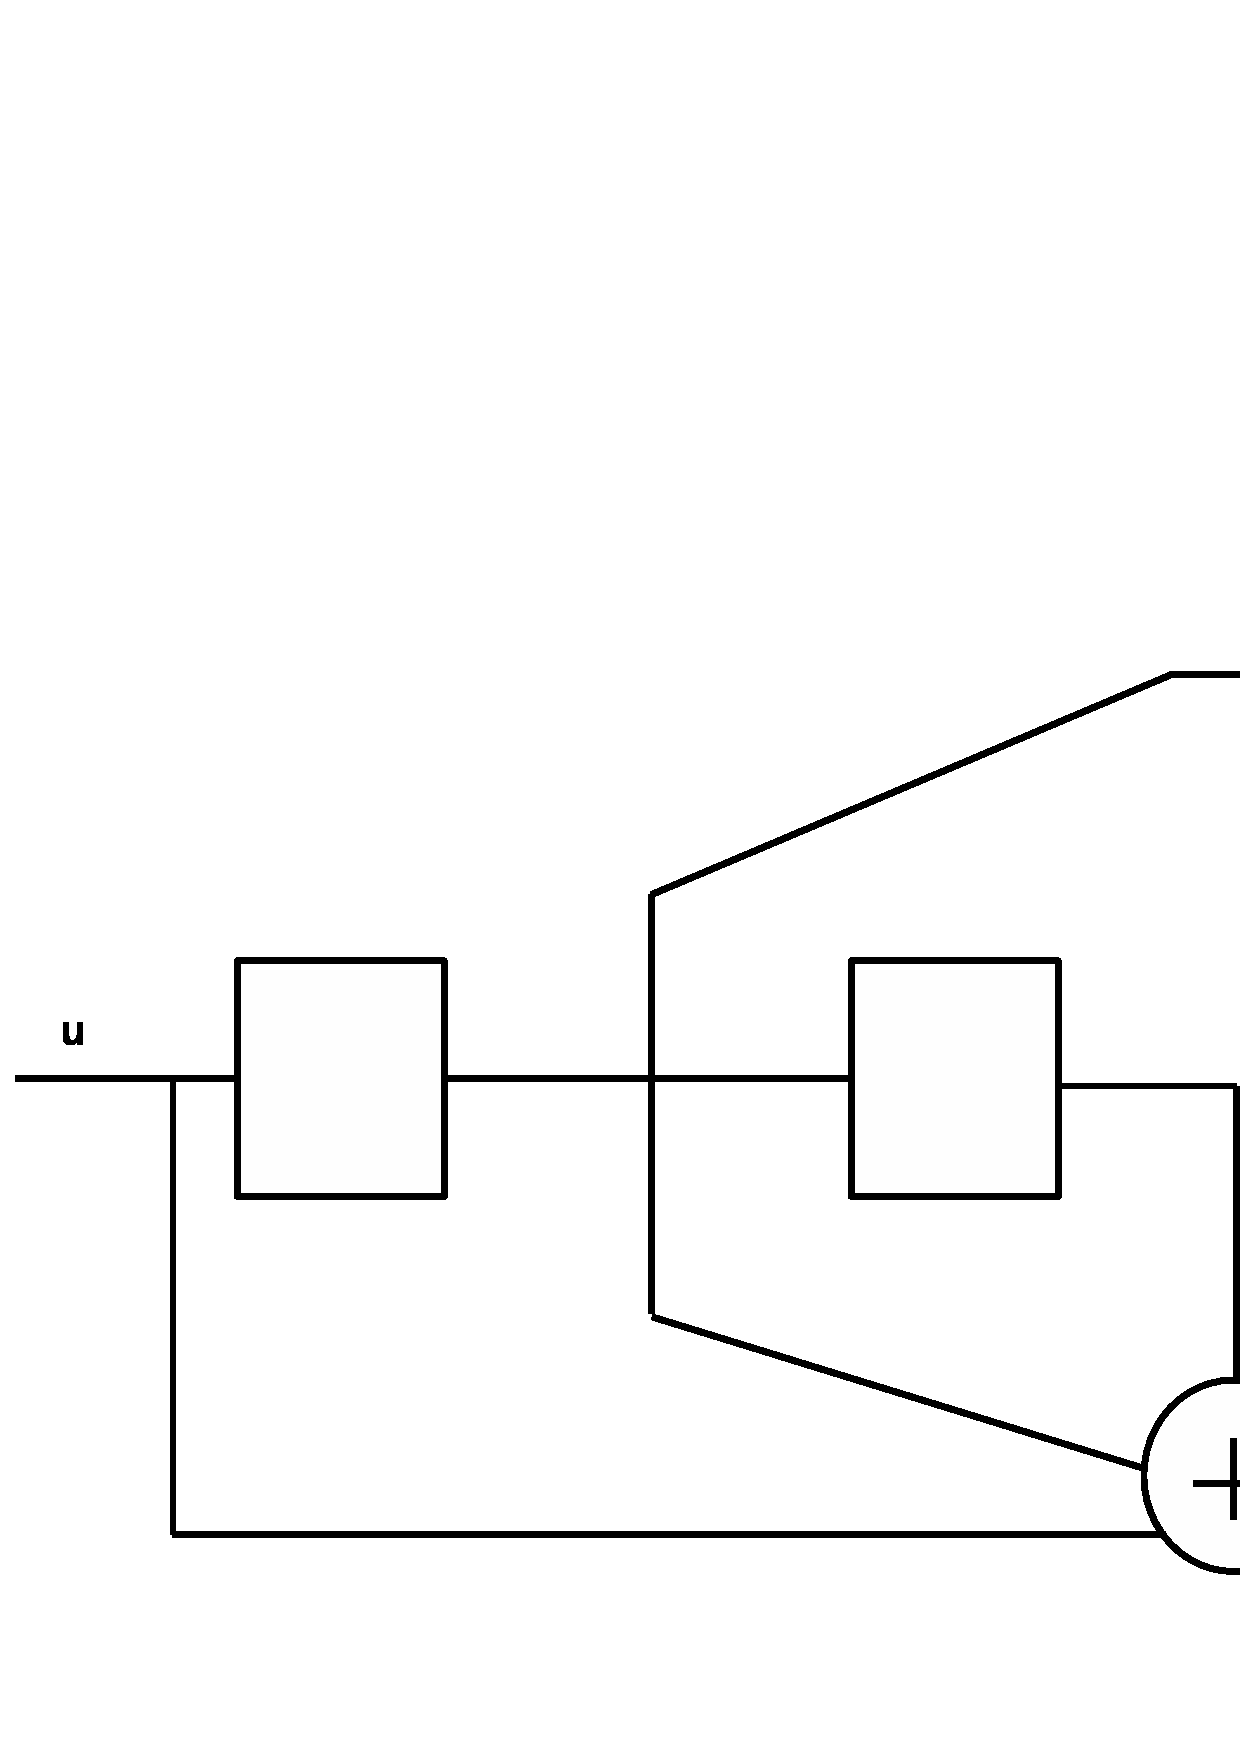
\includegraphics[width=0.4\textwidth]{enc}
%\caption{Feedforward encoder for the specified convolutional code of memory order 2}
%\label{enc}
%\end{figure}

\begin{figure}
\centering
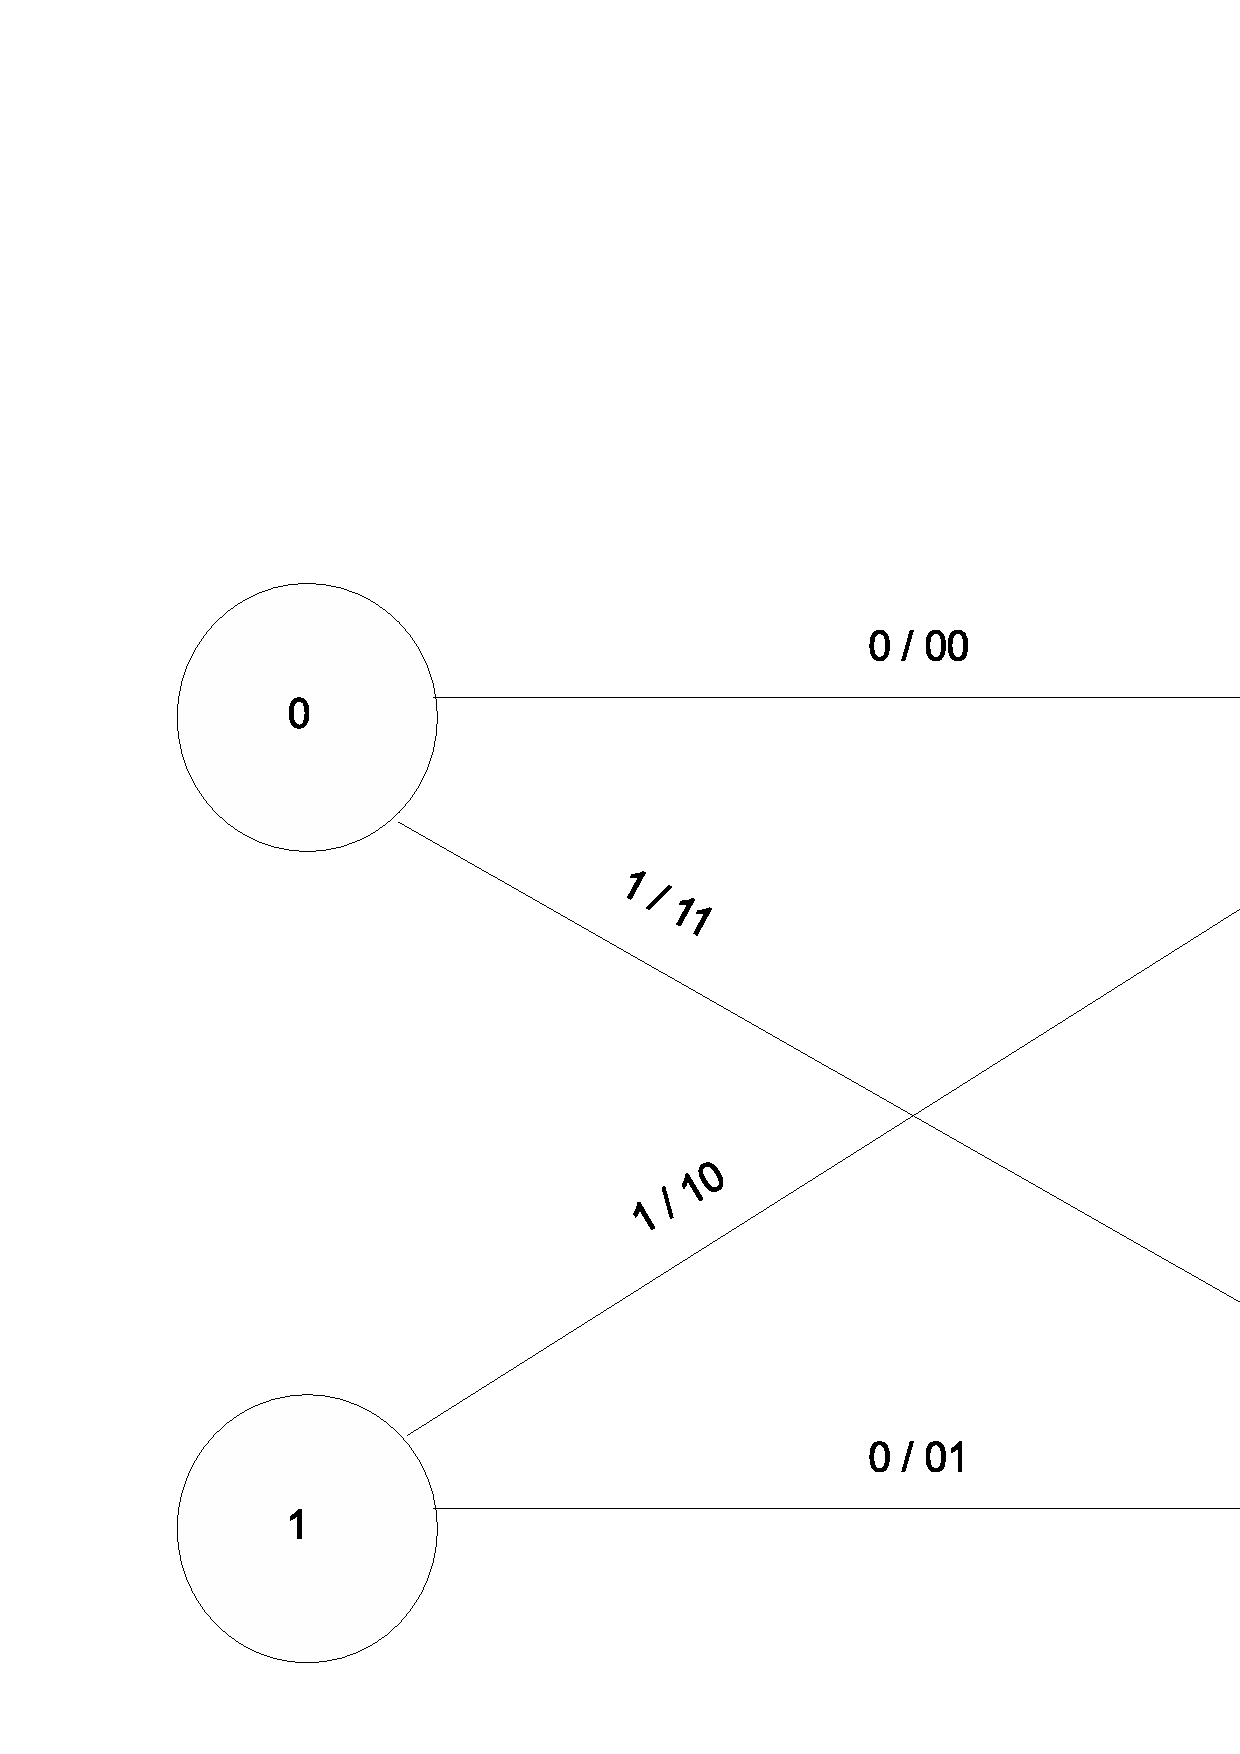
\includegraphics[width=0.5\textwidth]{images/state}
\caption{State Diagram for the convolutional code}
\label{state}
\end{figure}

For the decoding, we assume the all-zero input message. We pass it through the trellis encoder to obtain the output. 
The BCJR algorithm implements a bitwise-MAP rule. Unlike the Viterbi case, where we sent one long codeword, here we send many many blocks of small length codewords. The message length used was $k=7$. 
\\ \\
For code simplicity, we store 2 arrays, one for the state-nextstate-output relations for input 0, and one for input 1. For the BCJR algorithm, it also makes sense to store the reverse state map (given a state and an input, find the previous state and output).
\\ \\
We then use BPSK modulation to obtain the codeword sent through the channel. We use the code in \cite{AWGN} to simulate the AWGN channel for a given SNR. 



\section{BCJR Decoder} 

We implemented the Max-log-MAP decoding algorithm as shown in \cite{BCJR}. We first computed the branch metrics $\gamma^*_l(s,s')=\log \gamma_l(s,s') = \log p(s,r_l | s')$ for all branches in all iterations. 
\\ \\
We then do a forward trellis parse to compute all the $\alpha^*_l(s') = \log p(s', r_{t<l}) $ as a maximization based on previous $(\gamma^*,\alpha^*)$. We then use a bckward trellis parse ( using \textit{prev\_state} as our trellis ) to compute $\beta^*_l(s) = \log p(r_{t<l} | s)$ based on forward looking $(\gamma^*,\beta^*)$. The max-log map rule helps us keep each of the terms small, as we have a neat way to evaluate $\log(e^x + e^y)$
\\ \\
Finally, we calculate the aposteriori-probabilities (bit-LLRs) and make a decision on each bit. For every bit, we need to look at all possible state transitions  with $0,1$-input, and factor all of them into the aposteriori expression. Note that since we are making bit-decisions, there is no guarantee we get a codeword, and so we compute \textbf{Block Error} probability (instead of bit-error rate).
\\ \\
For a given SNR, we send about $5*10^4$ blocks of small length codewords. We run these through the BCJR algorithm. If the received vector does not decode correctly to the all-zero message vector, we add it to the count of block errors. In this way, we generate the Block Error Probability for each SNR. The script to implement this is \textbf{bcjr.m}.
\\ \\
Figure (\ref{ber}) shows the Block Error Probability curve for uncoded transmission over BPSK-AWGN, and that of the BCJR decoder. 
\pagebreak
\begin{figure}
\centering
\includegraphics[width=0.8\textwidth]{images/ber}
\caption{Comparison of Block error rate-SNR curves for the BCJR Decoder, and Uncoded BPSK transmission}
\label{ber}
\end{figure}

\begin{thebibliography}{155}
\bibitem{AWGN}
AWGN Generation in MATLAB \textit{addAWGN.m} - \\
http://stackoverflow.com/questions/23690766/proper-way-to-add-noise-to-signal

\bibitem{BCJR}
Presentation on the BCJR algorithm - \\
http://site.iugaza.edu.ps/ahdrouss/files/2011/03/SOVA-and-BCJR.pdf
\end{thebibliography}




\end{document}

